\begin{figure}[htbp]
	\centering
	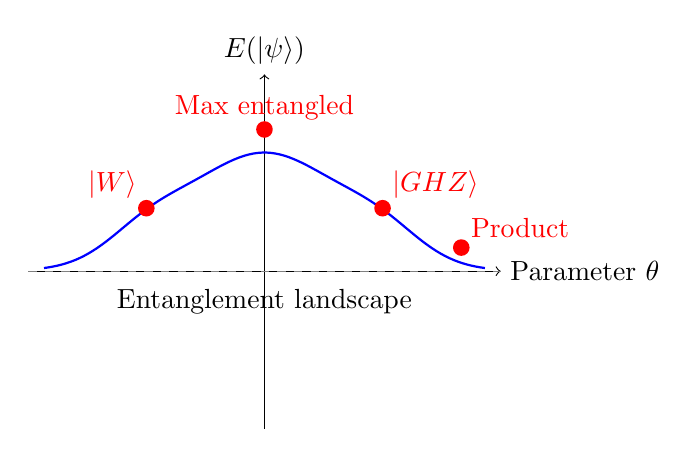
\begin{tikzpicture}
		\draw[->] (-3,0) -- (3,0) node[right] {Parameter $\theta$};
		\draw[->] (0,-2) -- (0,2.5) node[above] {$E(|\psi\rangle)$};

		\draw[thick, blue, domain=-2.8:2.8, samples=100] plot (\x, {1.5*exp(-\x*\x/2) + 0.3*exp(-(\x-1.5)*(\x-1.5)/0.5) + 0.3*exp(-(\x+1.5)*(\x+1.5)/0.5)});

		\fill[red] (1.5,0.8) circle (3pt) node[above right] {$|\text{GHZ}\rangle$};
		\fill[red] (-1.5,0.8) circle (3pt) node[above left] {$|W\rangle$};
		\fill[red] (0,1.8) circle (3pt) node[above] {Max entangled};
		\fill[red] (2.5,0.3) circle (3pt) node[above right] {Product};

		\draw[dashed, gray] (-3,0) -- (3,0);
		\node[below] at (0,-0.1) {Entanglement landscape};

	\end{tikzpicture}
	\caption{Entanglement landscape visualization using the Great Deluge Algorithm. Peaks correspond to highly entangled states (GHZ, W), valleys to product states. The algorithm floods this landscape to identify maximally entangled configurations. Great Deluge Algorithm: 1. Initialize random states, 2. Project to nearest peak, 3. Water level rises, 4. Find highly entangled states.}
	\label{fig:entanglement-landscape}
\end{figure}
